\documentclass{beamer}
\usepackage{graphicx}
%\usepackage{tikz}
%\usetikzlibrary{decorations.markings,arrows}
\usetheme[numbering=none]{metropolis}
\title{Functional Geometry Description of Escher's Fish}
\date{Feb 1, 2017}
\author{Milton Mazzarri}
\institute{Houston Elixir Meetup}
\begin{document}
    \maketitle

    \section{Introduction}

    \begin{frame}{Square Limit}

        \begin{figure}
           \centering
            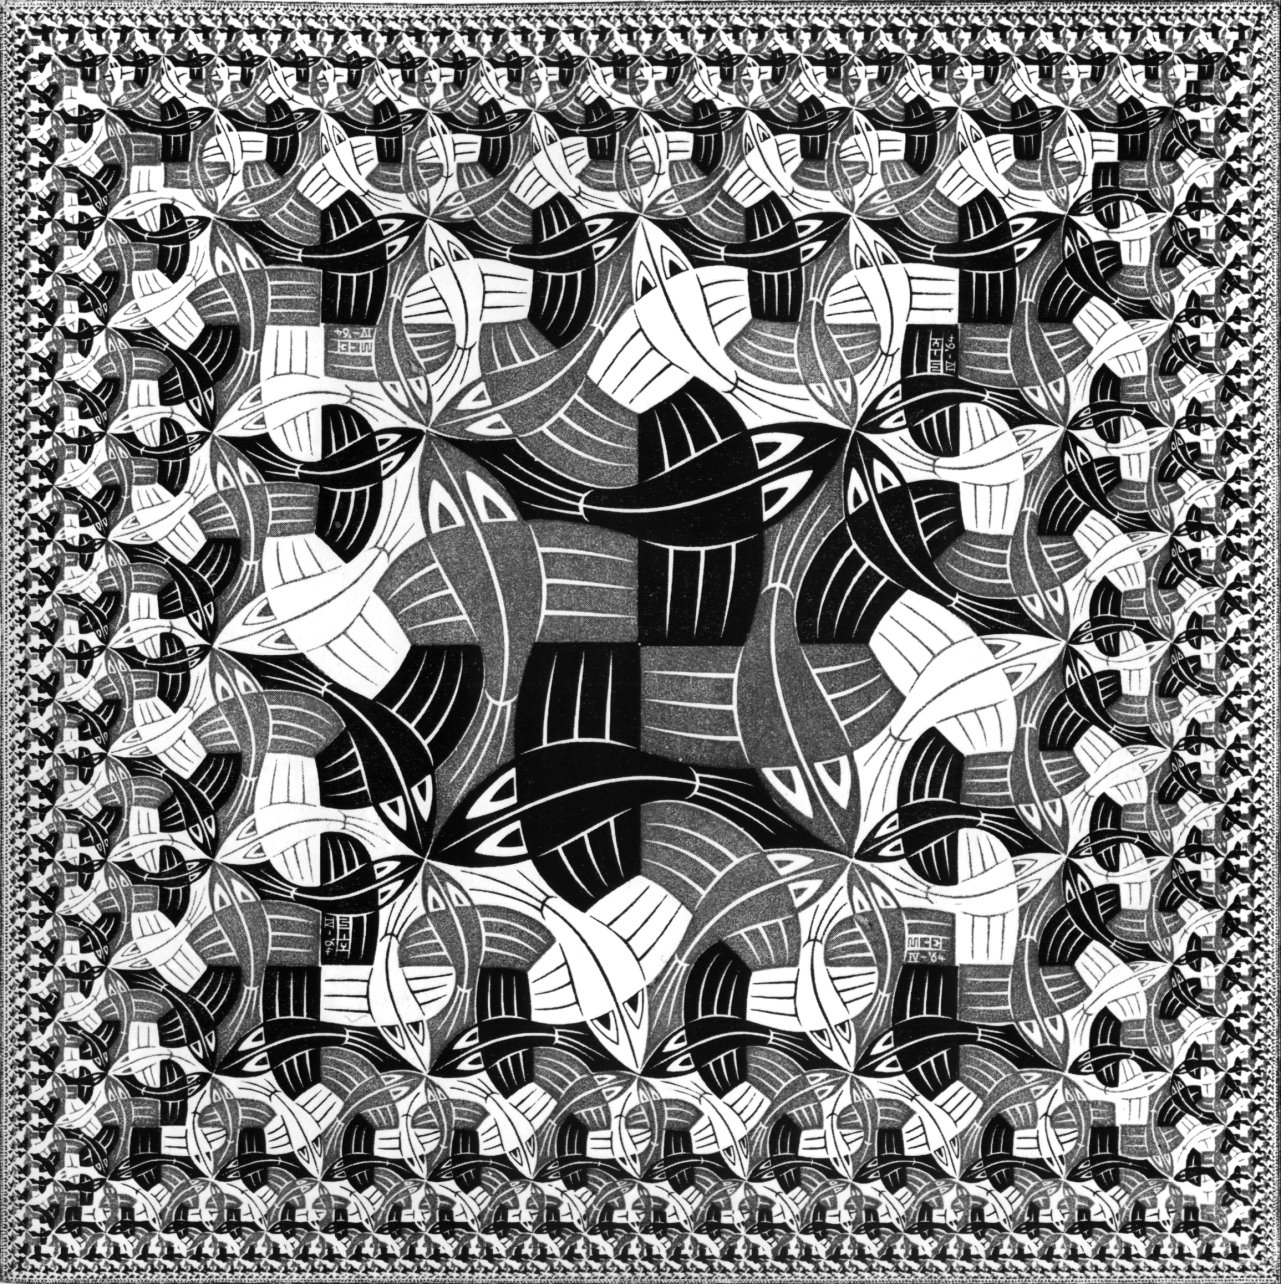
\includegraphics[width=0.5\textwidth]{./figs/square-limit}
            \caption{M.C. Escher's Square Limit}
            \label{fig:square_limit}
        \end{figure}
        {\footnotesize Source: \url{https://www.wikiart.org/en/m-c-escher/square-limit}}
    \end{frame}

    \begin{frame}{Functional Geometry}
        Functional Geometry is a paper by Peter Henderson\cite{Henderson82,Henderson02}, which deconstructs the M.C. Escher woodcut ``Square Limit''.
        \begin{quote}
            A picture is an example of a complex object that can be described
            in terms of its parts. Yet a picture needs to be rendered on a
            printer or a screen by a device that expects to be given a sequence
            of commands. Programming that sequence of commands directly is much
            harder than having an application generate the commands
            automatically from the simpler, denotational description.
        \end{quote}
    \end{frame}

    \section{Basic Operations}

    \begin{frame}{f}
        \begin{alertblock}{Note}
        The image it is located within a frame, but we do not consider the frame to be part of the picture.
        \end{alertblock}

        \begin{figure}
            \centering
            
\includegraphics[width=0.35\textwidth]{./figs/basic/f}
            \caption{\footnotesize The value \texttt{f} denotes the picture of the letter F}
            \label{fig:f}
        \end{figure}

    \end{frame}

    \begin{frame}{Basic operations on pictures}

        \begin{itemize}
            \item $rot(picture) :: picture$
            \item $flip(picture) :: picture$
            \item $rot45(picture) :: picture$
            \item $above(picture, picture) :: picture$
            \item $beside(picture, picture) :: picture$
            \item $over(picture, picture) :: picture$
        \end{itemize}

    \end{frame}

    \begin{frame}{Rotation}
        Rotates a picture 90$^{\circ}$ anticlockwise.

        \begin{figure}
            \centering
            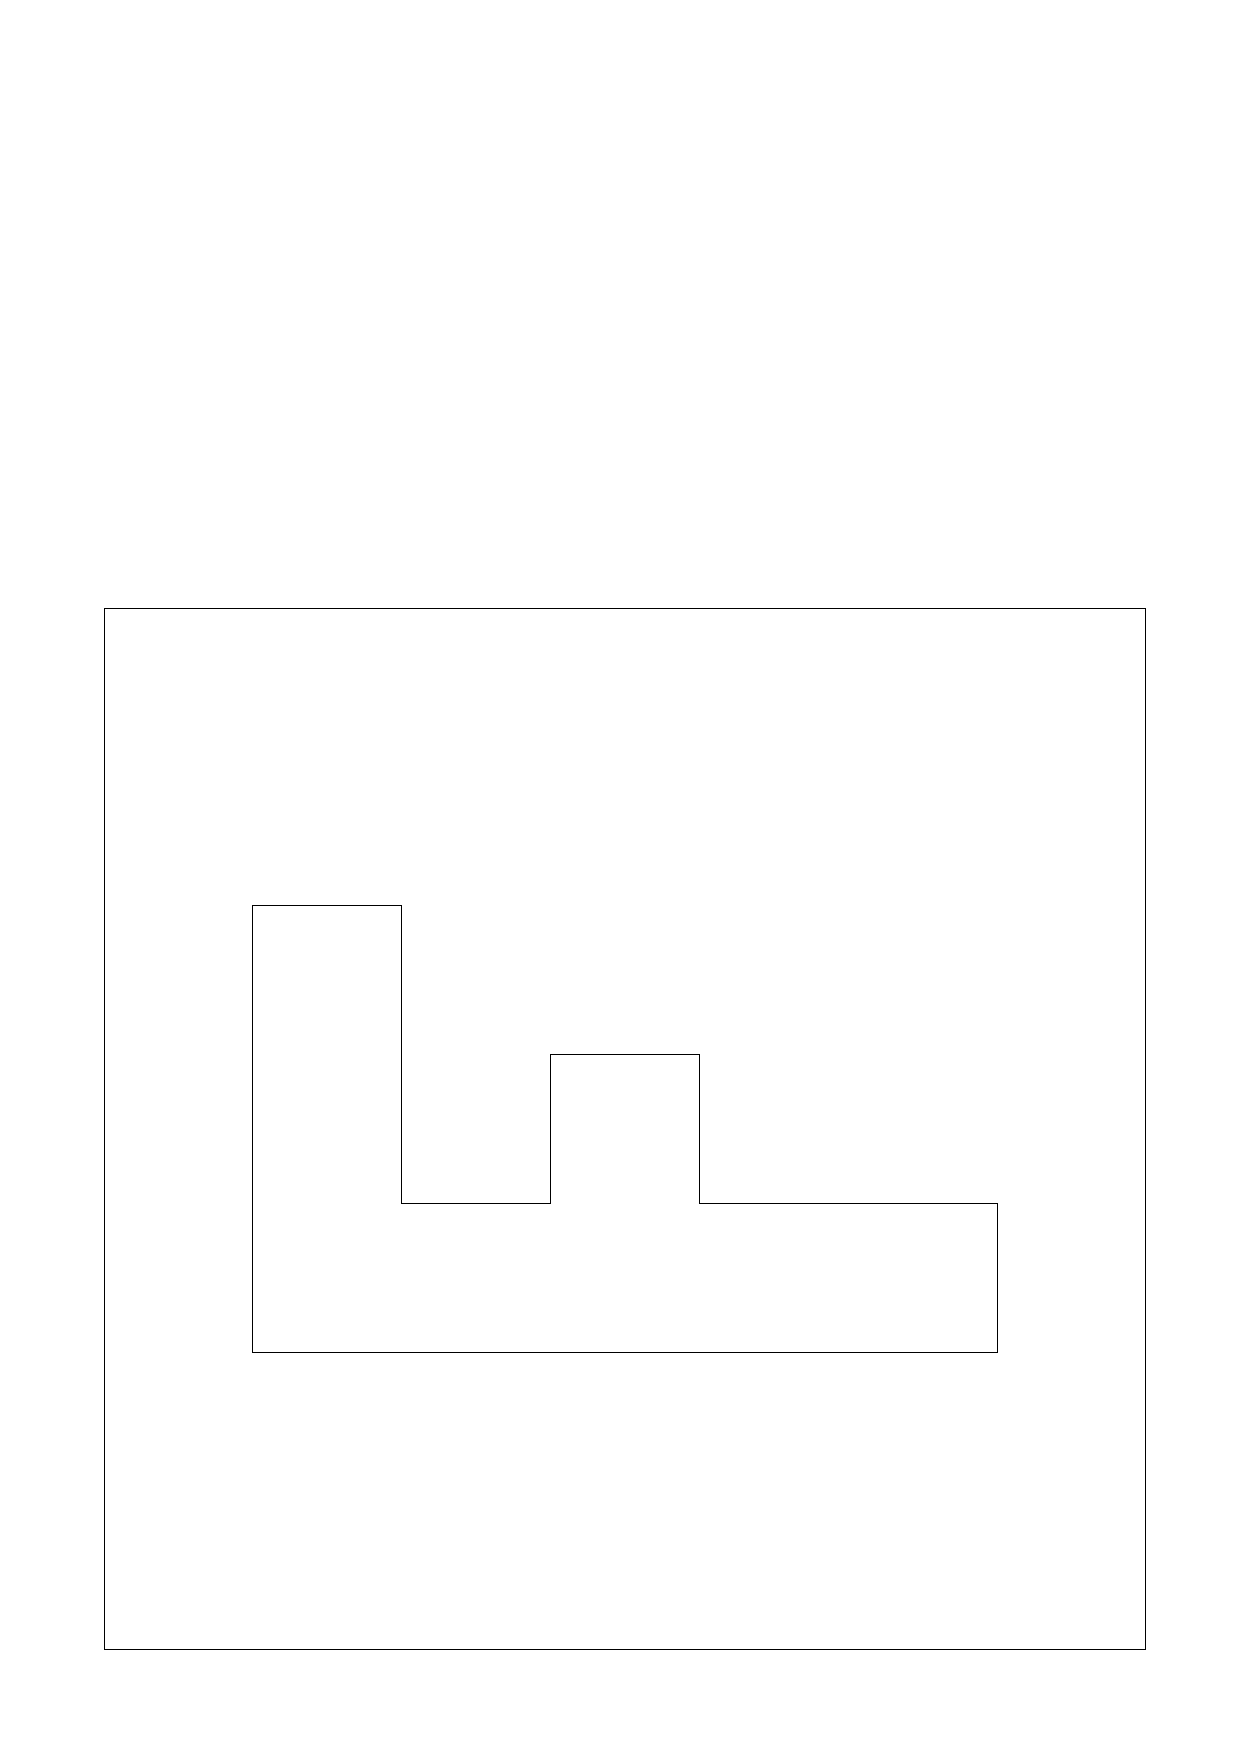
\includegraphics[width=0.4\textwidth]{./figs/basic/rot_f}
            \caption{\texttt{rot(f)}}
            \label{fig:rot_f}
        \end{figure}
    \end{frame}

    \begin{frame}{Flip}
    	Flip a picture through its vertical centre axis.

        \begin{figure}
            \centering
            
\includegraphics[width=0.4\textwidth]{./figs/basic/flip_f}
            \caption{\texttt{flip(f)}}
            \label{fig:flip_f}
        \end{figure}
    \end{frame}

    \begin{frame}{Rotation and Flip}

        \begin{figure}
            \centering
            
\includegraphics[width=0.4\textwidth]{./figs/basic/rot_flip_f}
            \caption{\texttt{rot(flip(f))}}
            \label{fig:rot_flip_f}
        \end{figure}
    \end{frame}

    \begin{frame}{Rotation 45$^{\circ}$}
    	Rotates a picture about its top left corner, through 45$^{\circ}$ anticlockwise.

        \begin{figure}
            \centering
            
\includegraphics[width=0.4\textwidth]{./figs/basic/rot45}
            \caption{\texttt{rot45(f)}}
            \label{fig:rot45}
        \end{figure}
    \end{frame}

    \begin{frame}{Above}
        \texttt{above(p, q)} is the picture that has \texttt{p} in the upper half
        of its locating box and \texttt{q} in the lower half.

        \begin{figure}
            \centering
            
\includegraphics[width=0.4\textwidth]{./figs/basic/above_f}
            \caption{\texttt{above(f, f)}}
            \label{fig:above}
        \end{figure}
    \end{frame}

    \begin{frame}{Beside}
        \texttt{beside(p, q)} is the picture that has \texttt{p} in the left half
        of its locating box and \texttt{q} in the right half.

        \begin{figure}
            \centering
            
\includegraphics[width=0.4\textwidth]{./figs/basic/beside_f}
            \caption{\texttt{beside(f, f)}}
            \label{fig:beside}
        \end{figure}
    \end{frame}

    \begin{frame}{above/beside combination}
        \begin{figure}
            \centering
            
\includegraphics[width=0.4\textwidth]{./figs/basic/above_beside_f}
            \caption{\texttt{above(beside(f, f) f)}}
            \label{fig:above_beside_f}
        \end{figure}
    \end{frame}

    \begin{frame}{Superposition}
        \begin{figure}
            \centering
            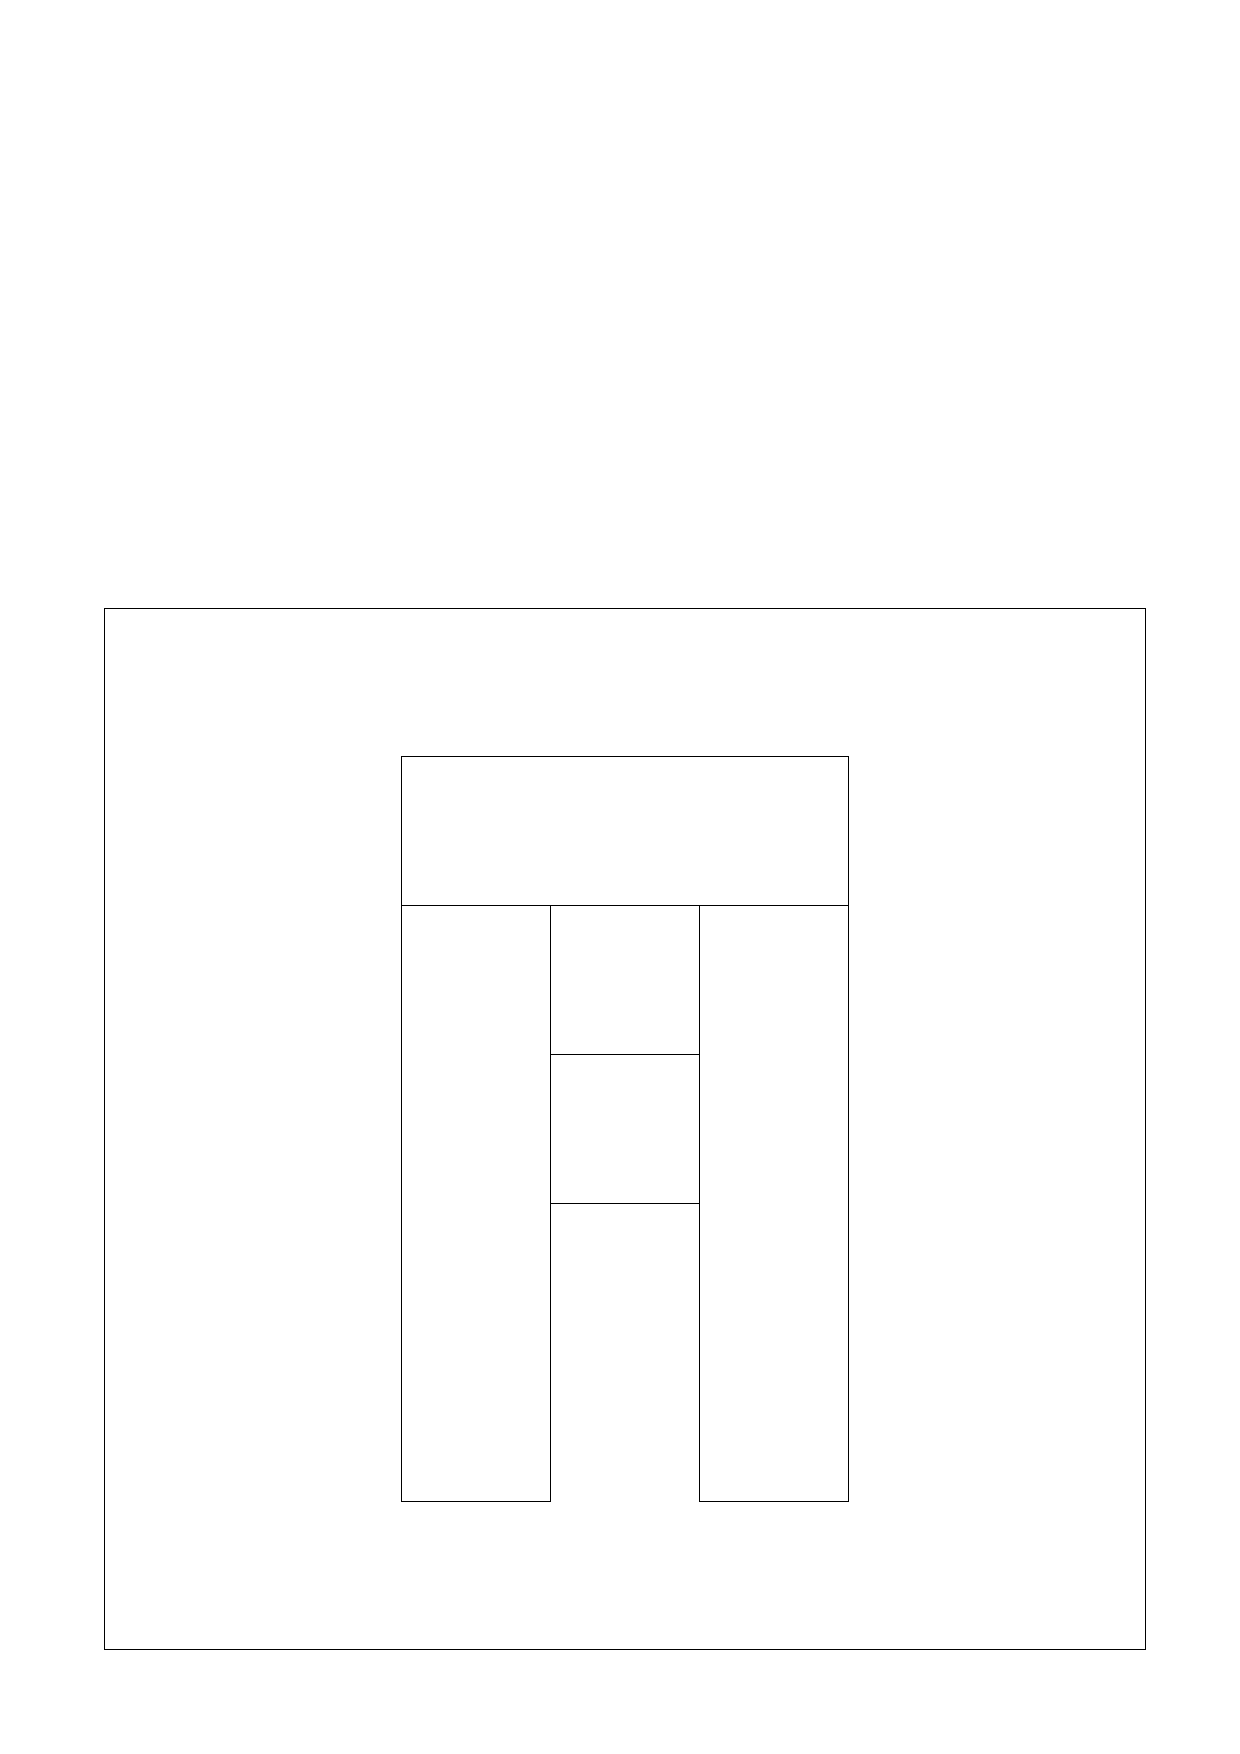
\includegraphics[width=0.4\textwidth]{./figs/basic/over}
            \caption{\texttt{over(f, flip(f))}}
            \label{fig:over_f}
        \end{figure}
    \end{frame}

    \section{Laws}

    \begin{frame}{Laws (Unit Test)}

        \begin{equation*}
        rot(rot(rot(rot(p)))) = p
        \end{equation*}

        \begin{equation*}
        rot(above(p, q)) = beside(rot(p), rot(q))
        \end{equation*}

        \begin{equation*}
        rot(beside(p, q)) = above(rot(q), rot(p))
        \end{equation*}

        \begin{equation*}
        flip(beside(p, q)) = beside(flip(q), flip(p))
        \end{equation*}
    \end{frame}

    \section{Square Limit}

    \begin{frame}{Basic patterns: p, q}

        \begin{columns}[T,onlytextwidth]
            \column{0.5\textwidth}
                \begin{figure}
                    \centering
                    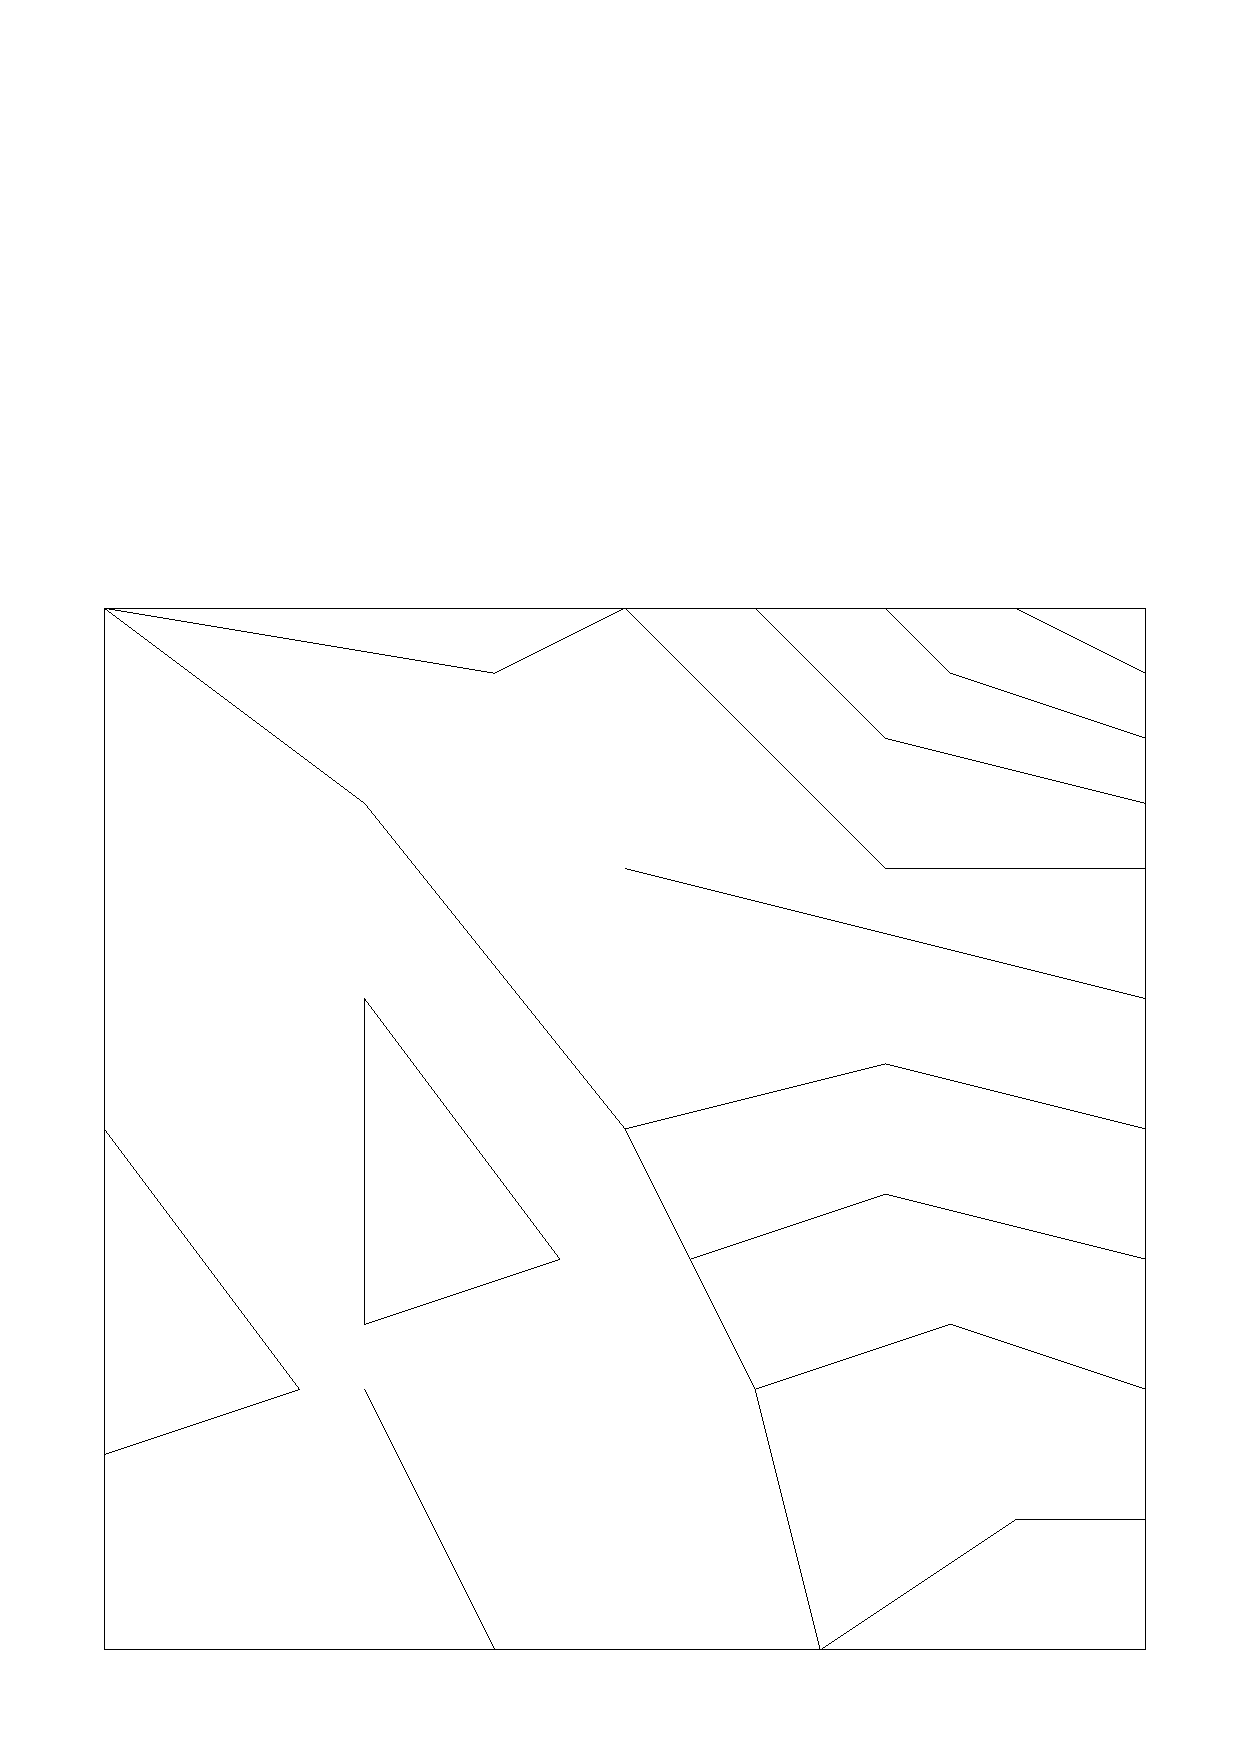
\includegraphics[width=0.5\textwidth]{./figs/fishes/p}
                    \caption{\texttt{p}}
                    \label{fig:p}
                \end{figure}

            \column{0.5\textwidth}
                \begin{figure}
                    \centering
                    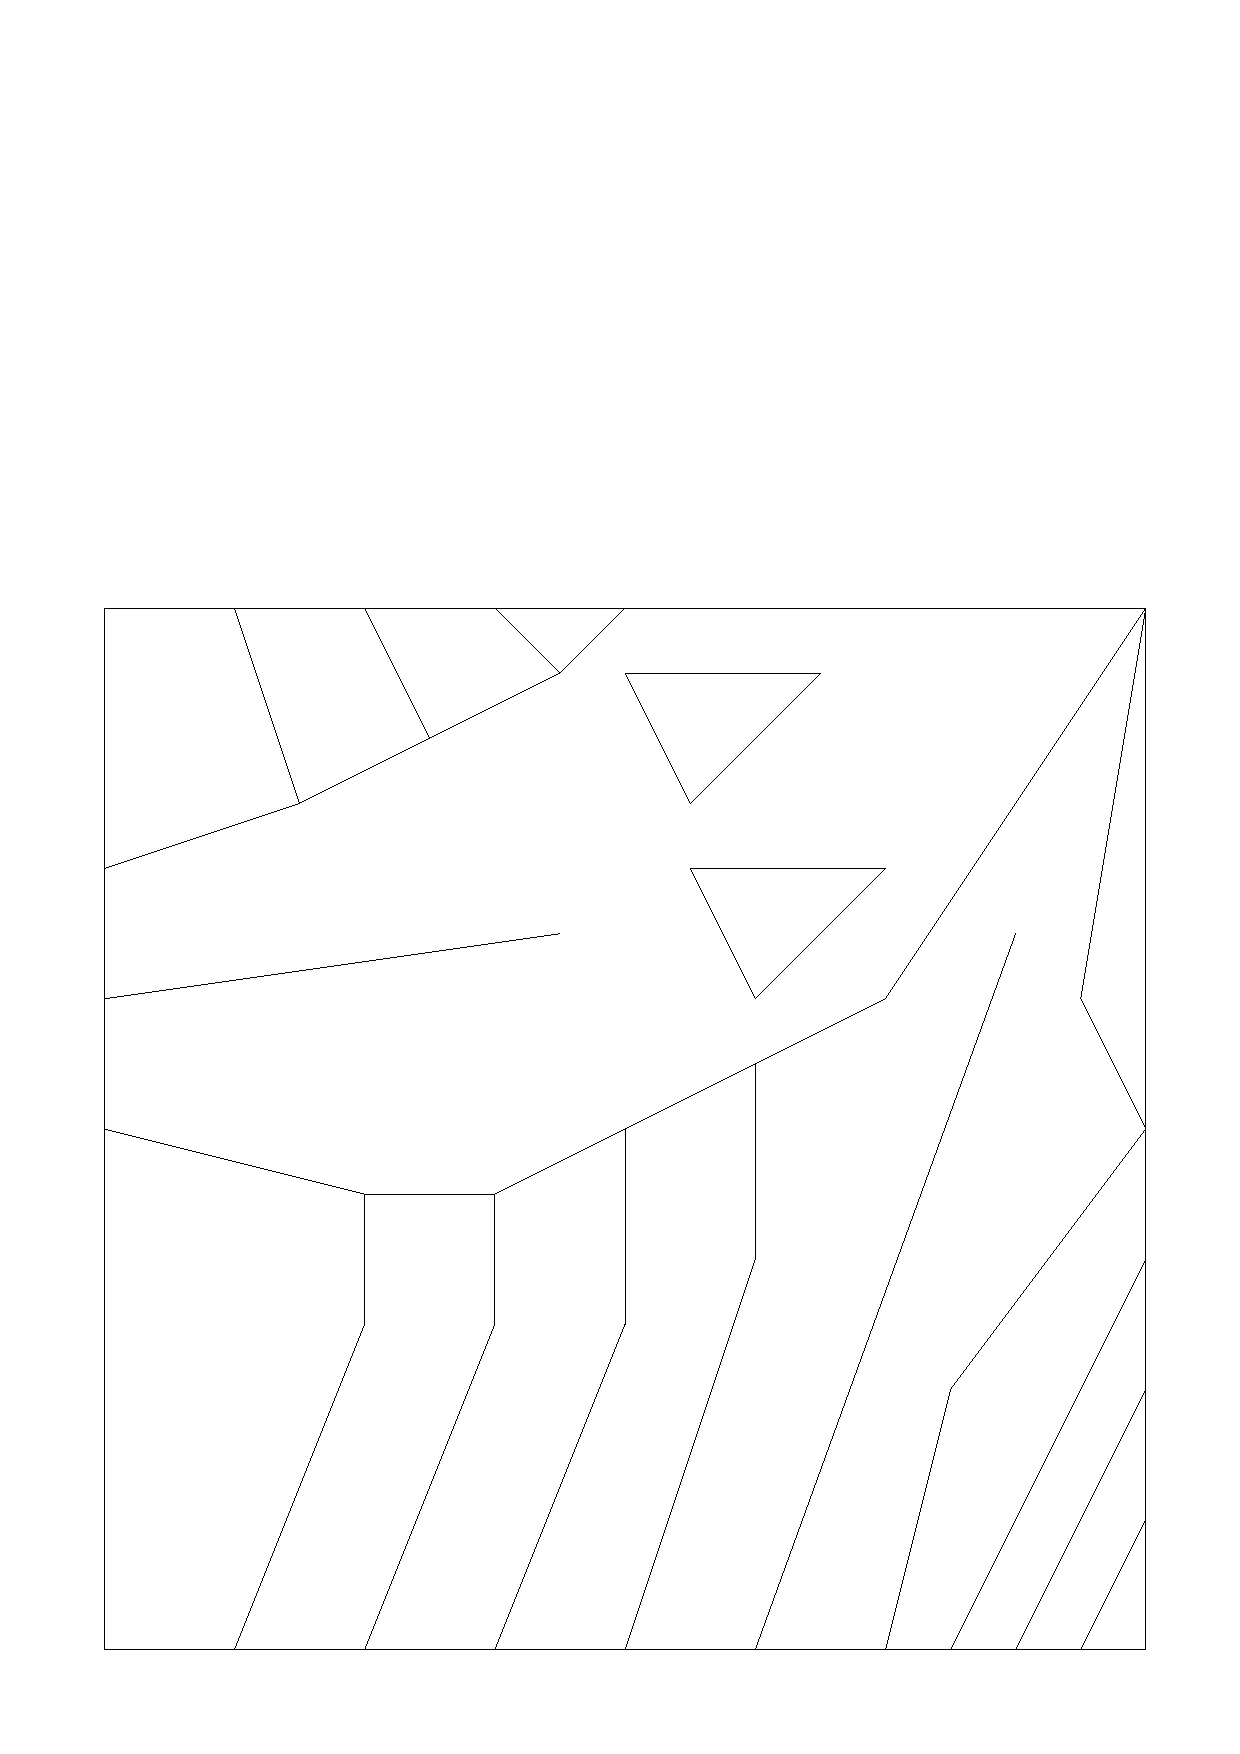
\includegraphics[width=0.5\textwidth]{./figs/fishes/q}
                    \caption{\texttt{q}}
                    \label{fig:q}
                \end{figure}

        \end{columns}

    \end{frame}

    \begin{frame}{Basic patterns: r, s}
        \begin{columns}[T,onlytextwidth]
            \column{0.5\textwidth}
                \begin{figure}
                    \centering
                    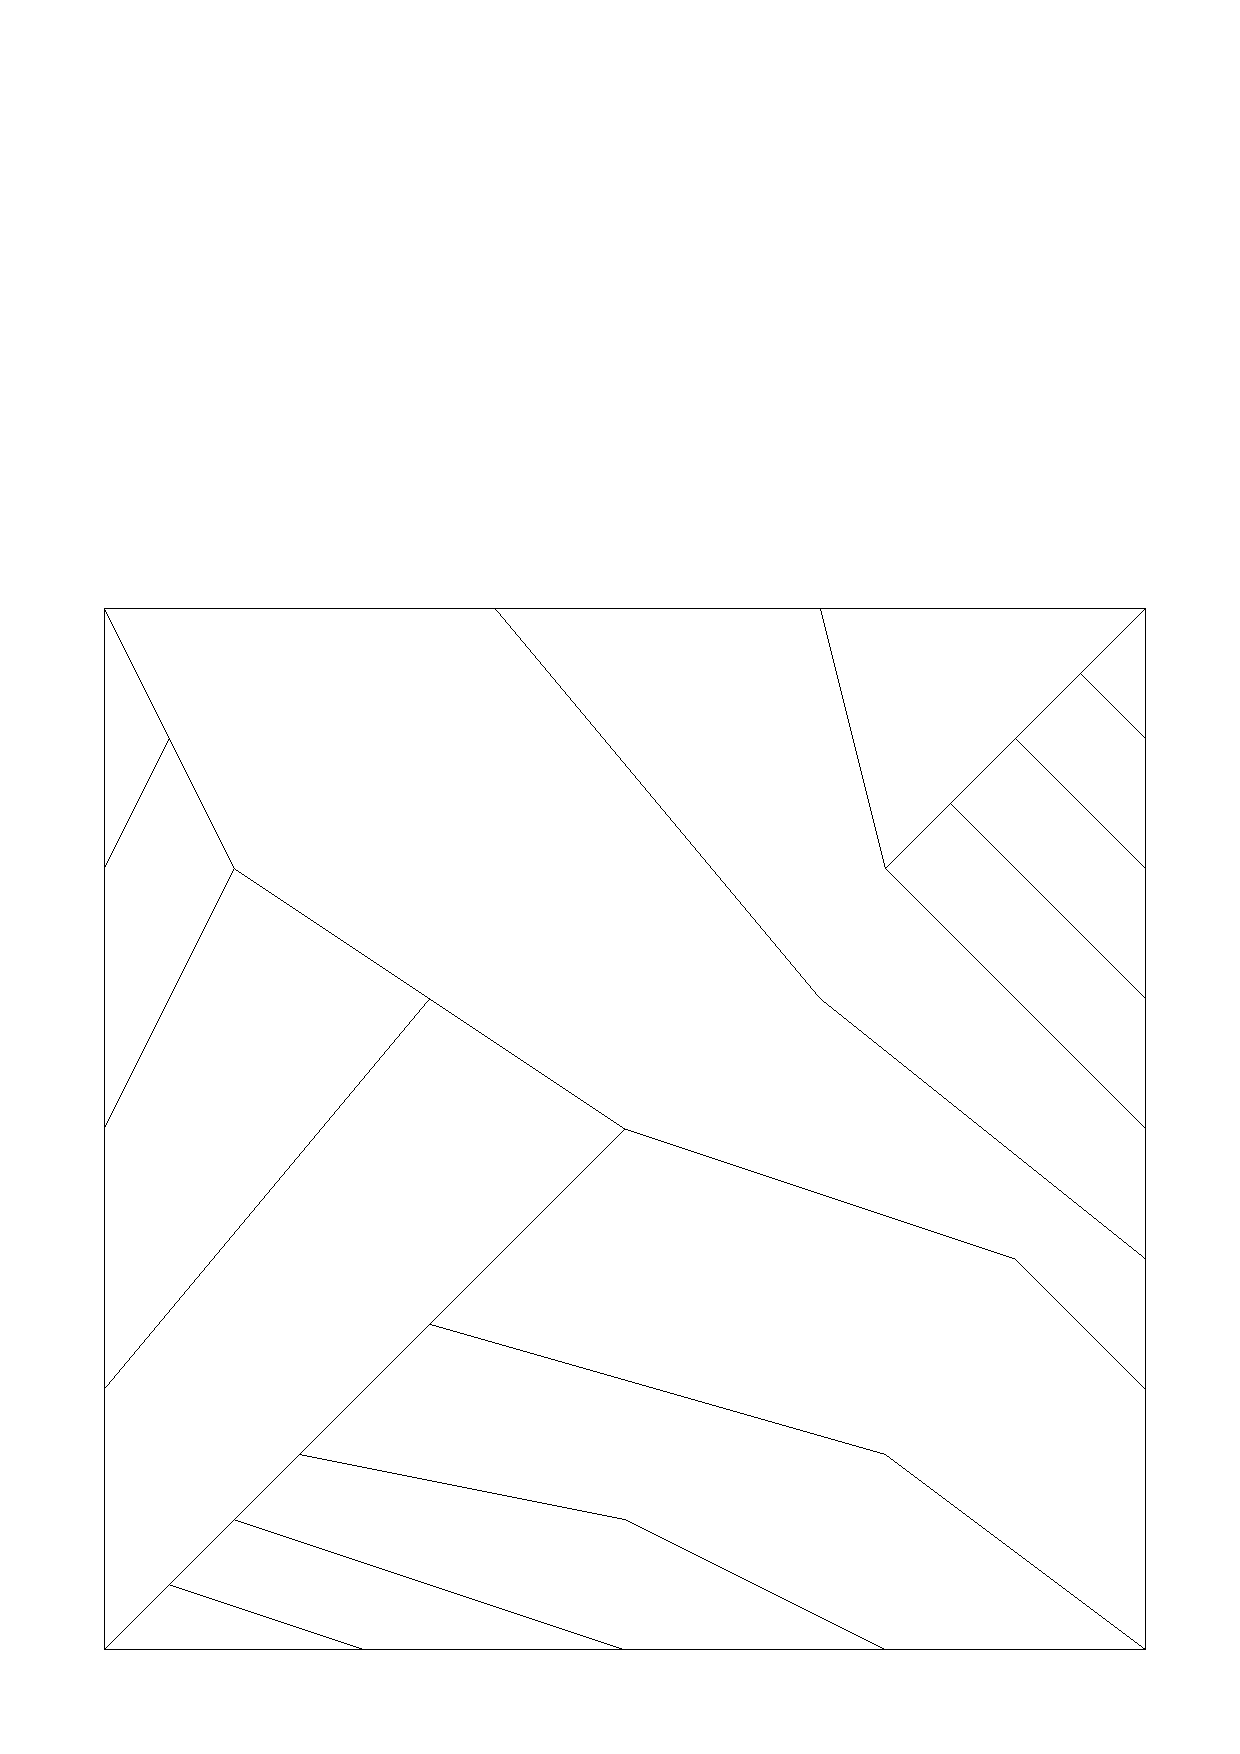
\includegraphics[width=0.5\textwidth]{./figs/fishes/r}
                    \caption{\texttt{r}}
                    \label{fig:r}
                \end{figure}

            \column{0.5\textwidth}
                \begin{figure}
                    \centering
                    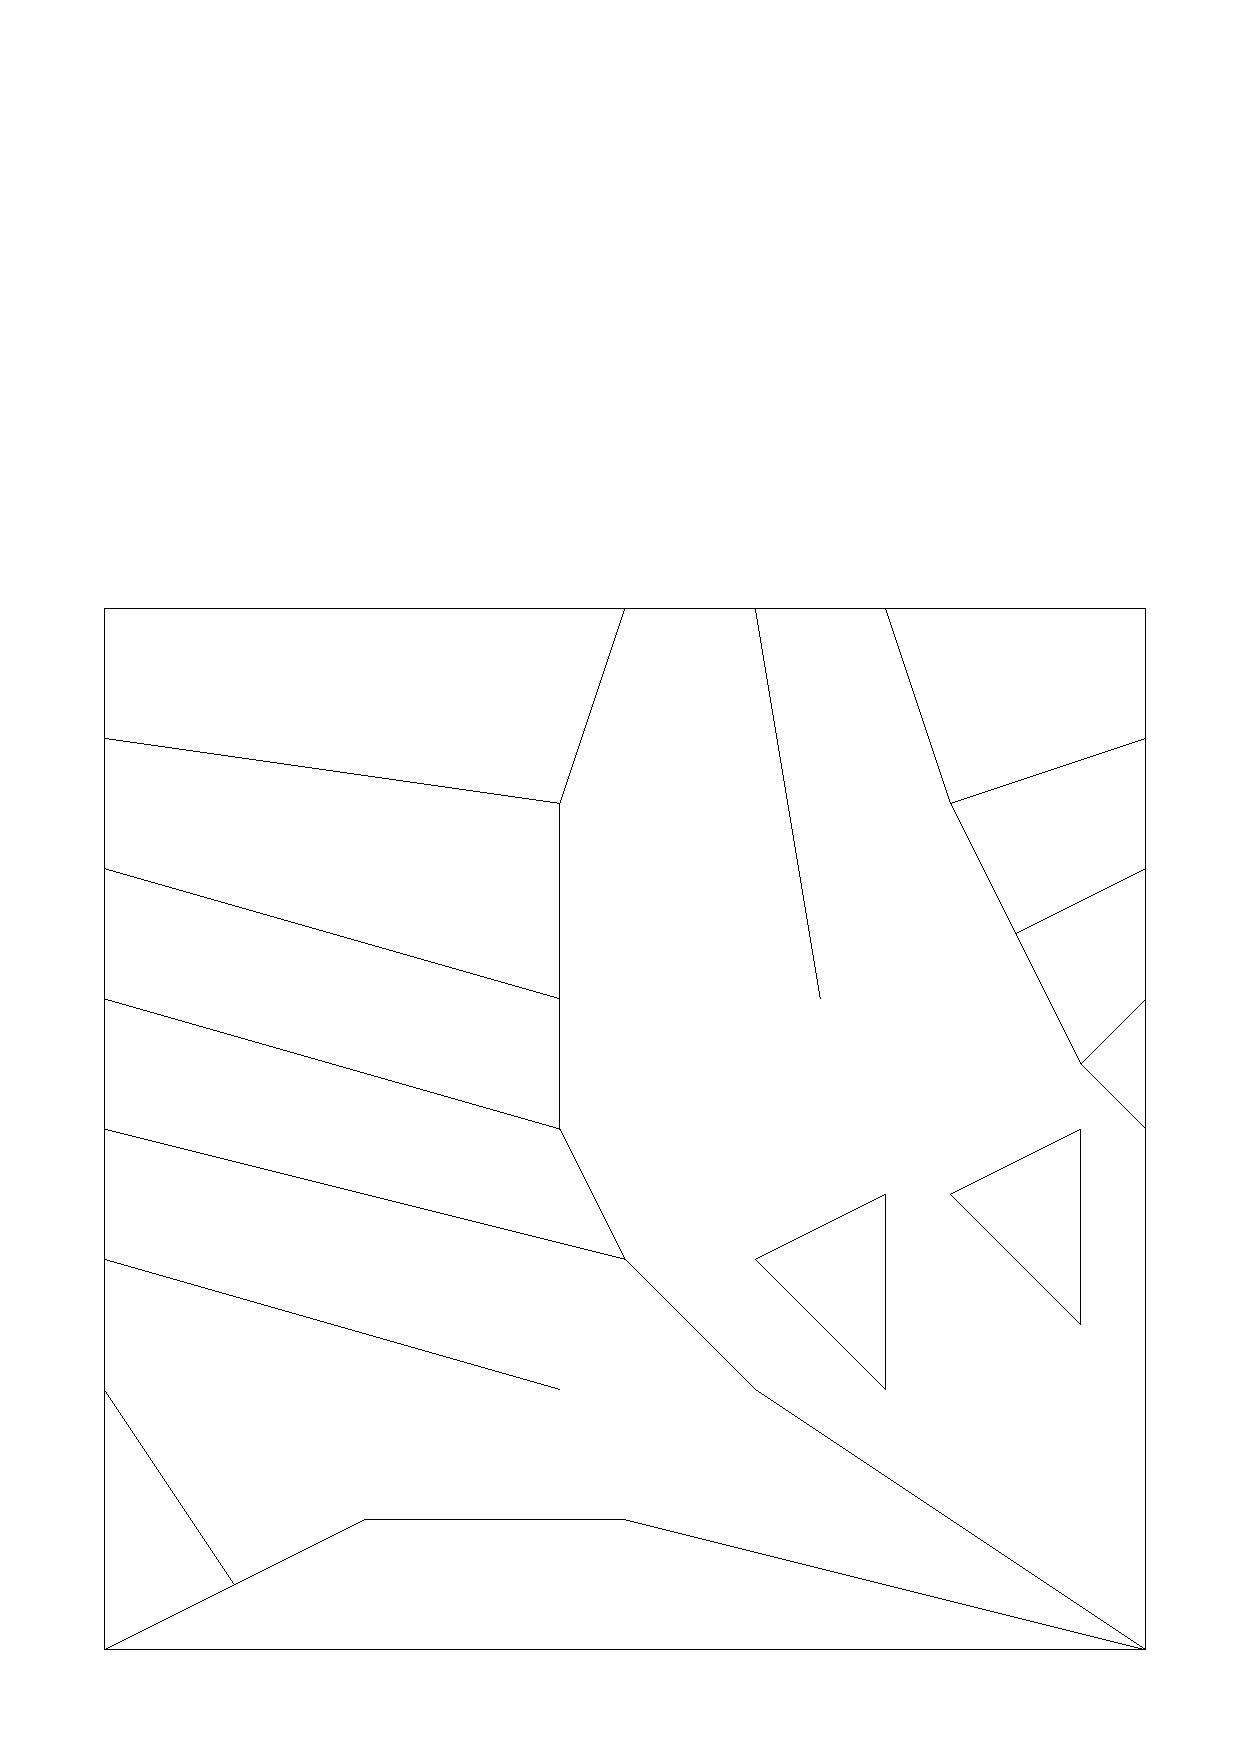
\includegraphics[width=0.5\textwidth]{./figs/fishes/s}
                    \caption{\texttt{s}}
                    \label{fig:s}
                \end{figure}
        \end{columns}

    \end{frame}

    \begin{frame}{t}

        \begin{figure}
            \centering
            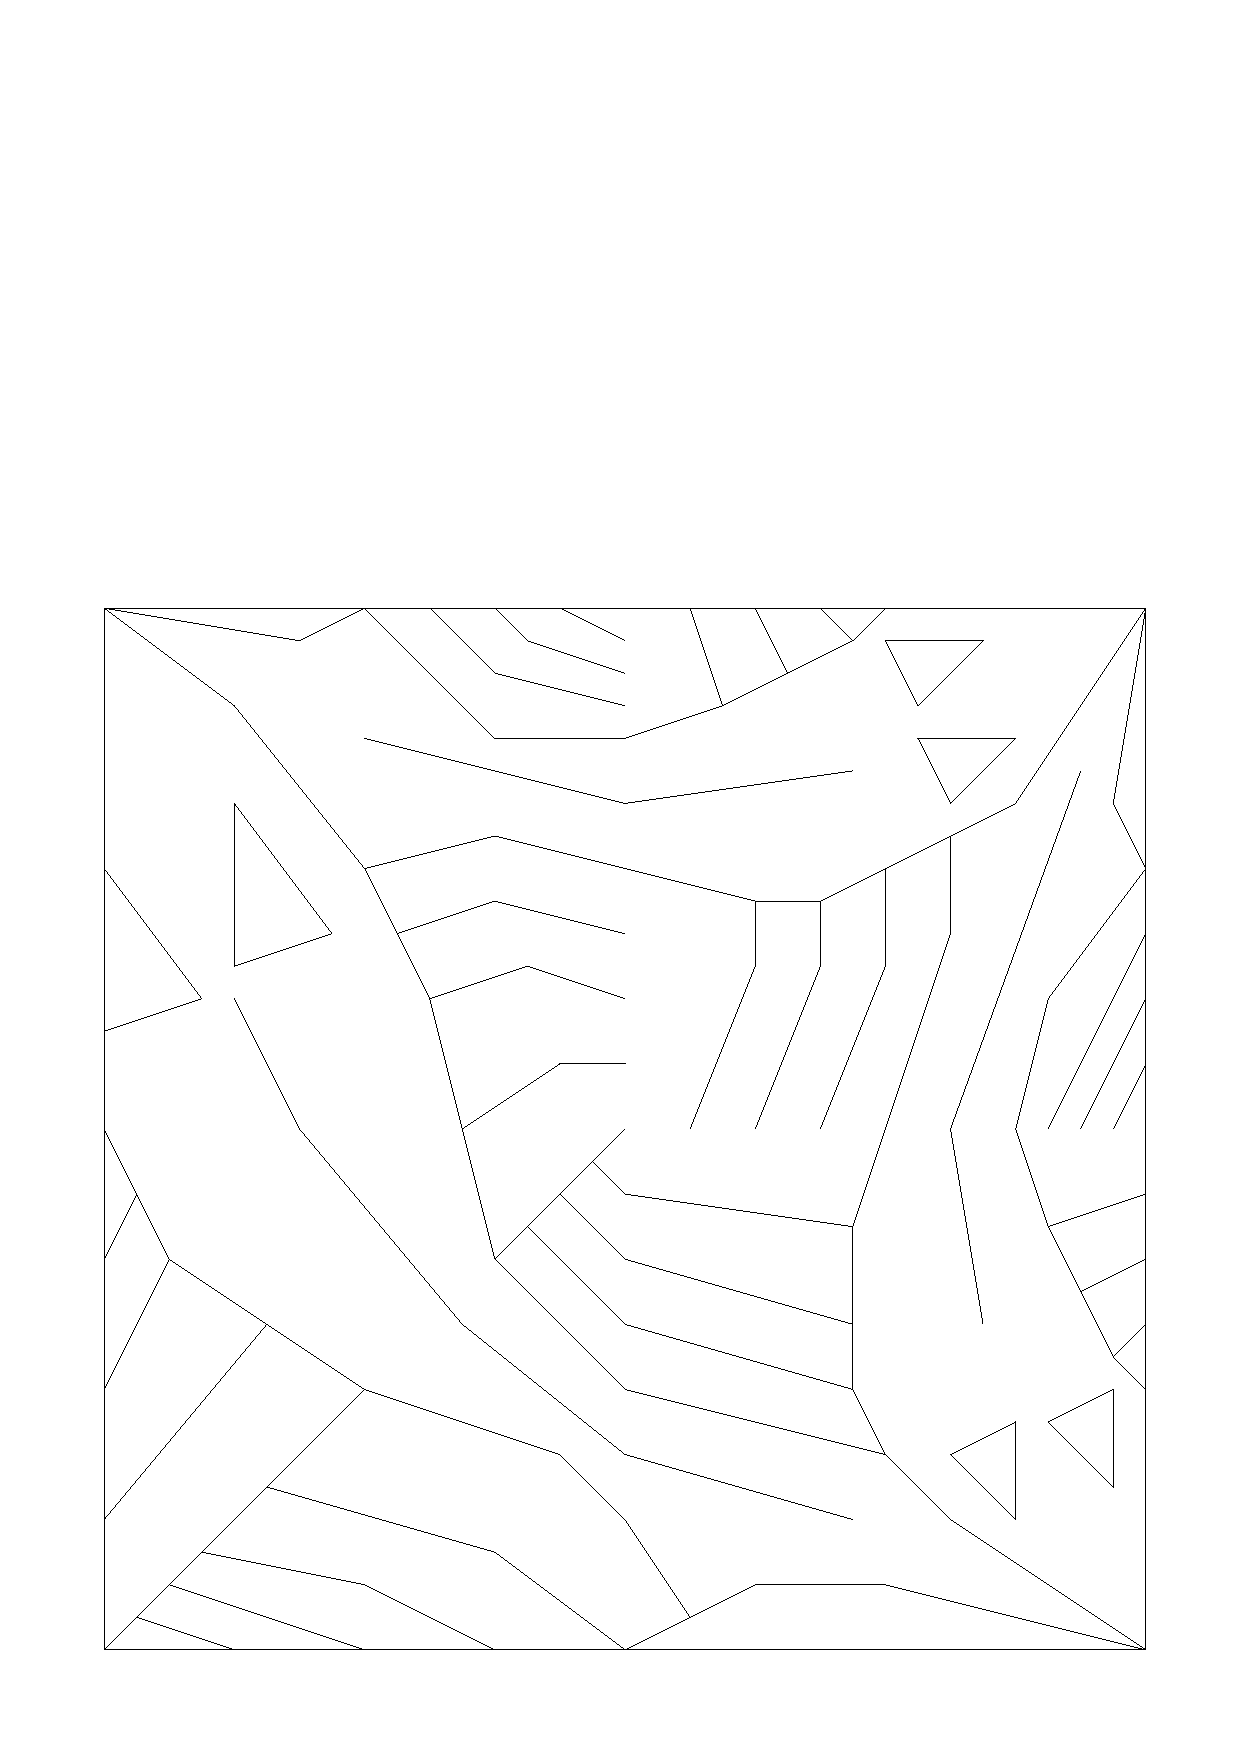
\includegraphics[width=0.5\textwidth]{./figs/fishes/t}
            \caption{\texttt{t = quartet(p, q, r, s)}}
            \label{fig:t}
        \end{figure}

    \end{frame}

    \begin{frame}{u}

        \begin{figure}
            \centering
            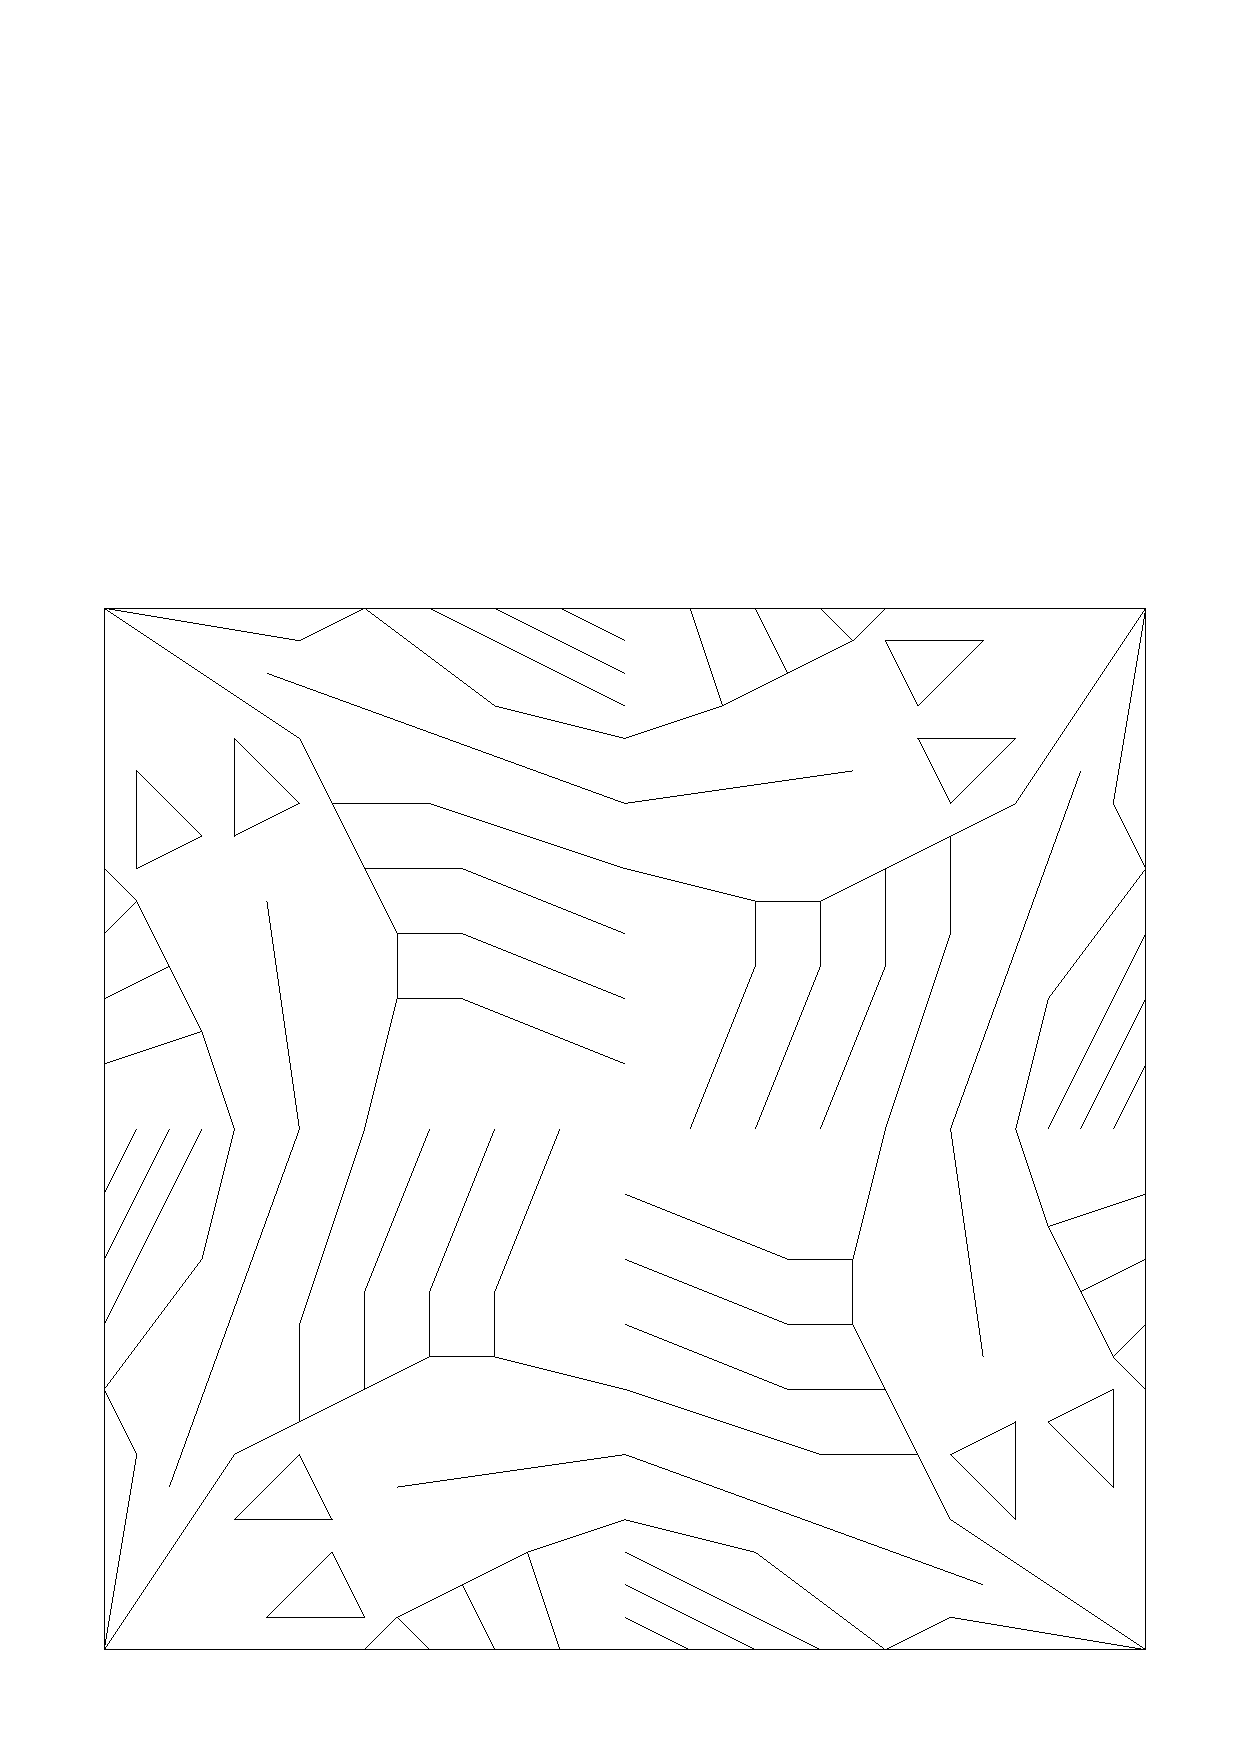
\includegraphics[width=0.5\textwidth]{./figs/fishes/u}
            \caption{\texttt{u = cycle(rot(q))}}
            \label{fig:u}
        \end{figure}

    \end{frame}

    \begin{frame}{side1}

        \begin{figure}
            \centering
            
\includegraphics[width=0.5\textwidth]{./figs/fishes/side1}
            \caption{\texttt{side1 = quartet(blank, blank, rot(t), t)}}
            \label{fig:side1}
        \end{figure}

    \end{frame}

   \begin{frame}{side2}

        \begin{figure}
            \centering
            
\includegraphics[width=0.5\textwidth]{./figs/fishes/side2}
            \caption{\texttt{side2 = quartet(side1, side1, rot(t), t)}}
            \label{fig:side2}
        \end{figure}

    \end{frame}

    \begin{frame}{corner1}

        \begin{figure}
            \centering
            
\includegraphics[width=0.5\textwidth]{./figs/fishes/corner1}
            \caption{\texttt{corner1 = quartet(blank, blank, blank, u)}}
            \label{fig:corner1}
        \end{figure}

    \end{frame}

    \begin{frame}{corner2}

        \begin{figure}
            \centering
            
\includegraphics[width=0.5\textwidth]{./figs/fishes/corner2}
            \caption{\footnotesize \texttt{corner2 = quartet(corner1, side1, rot(side1), u)}}
            \label{fig:corner2}
        \end{figure}

    \end{frame}

    \begin{frame}{pseudocorner}

        \begin{figure}
            \centering
            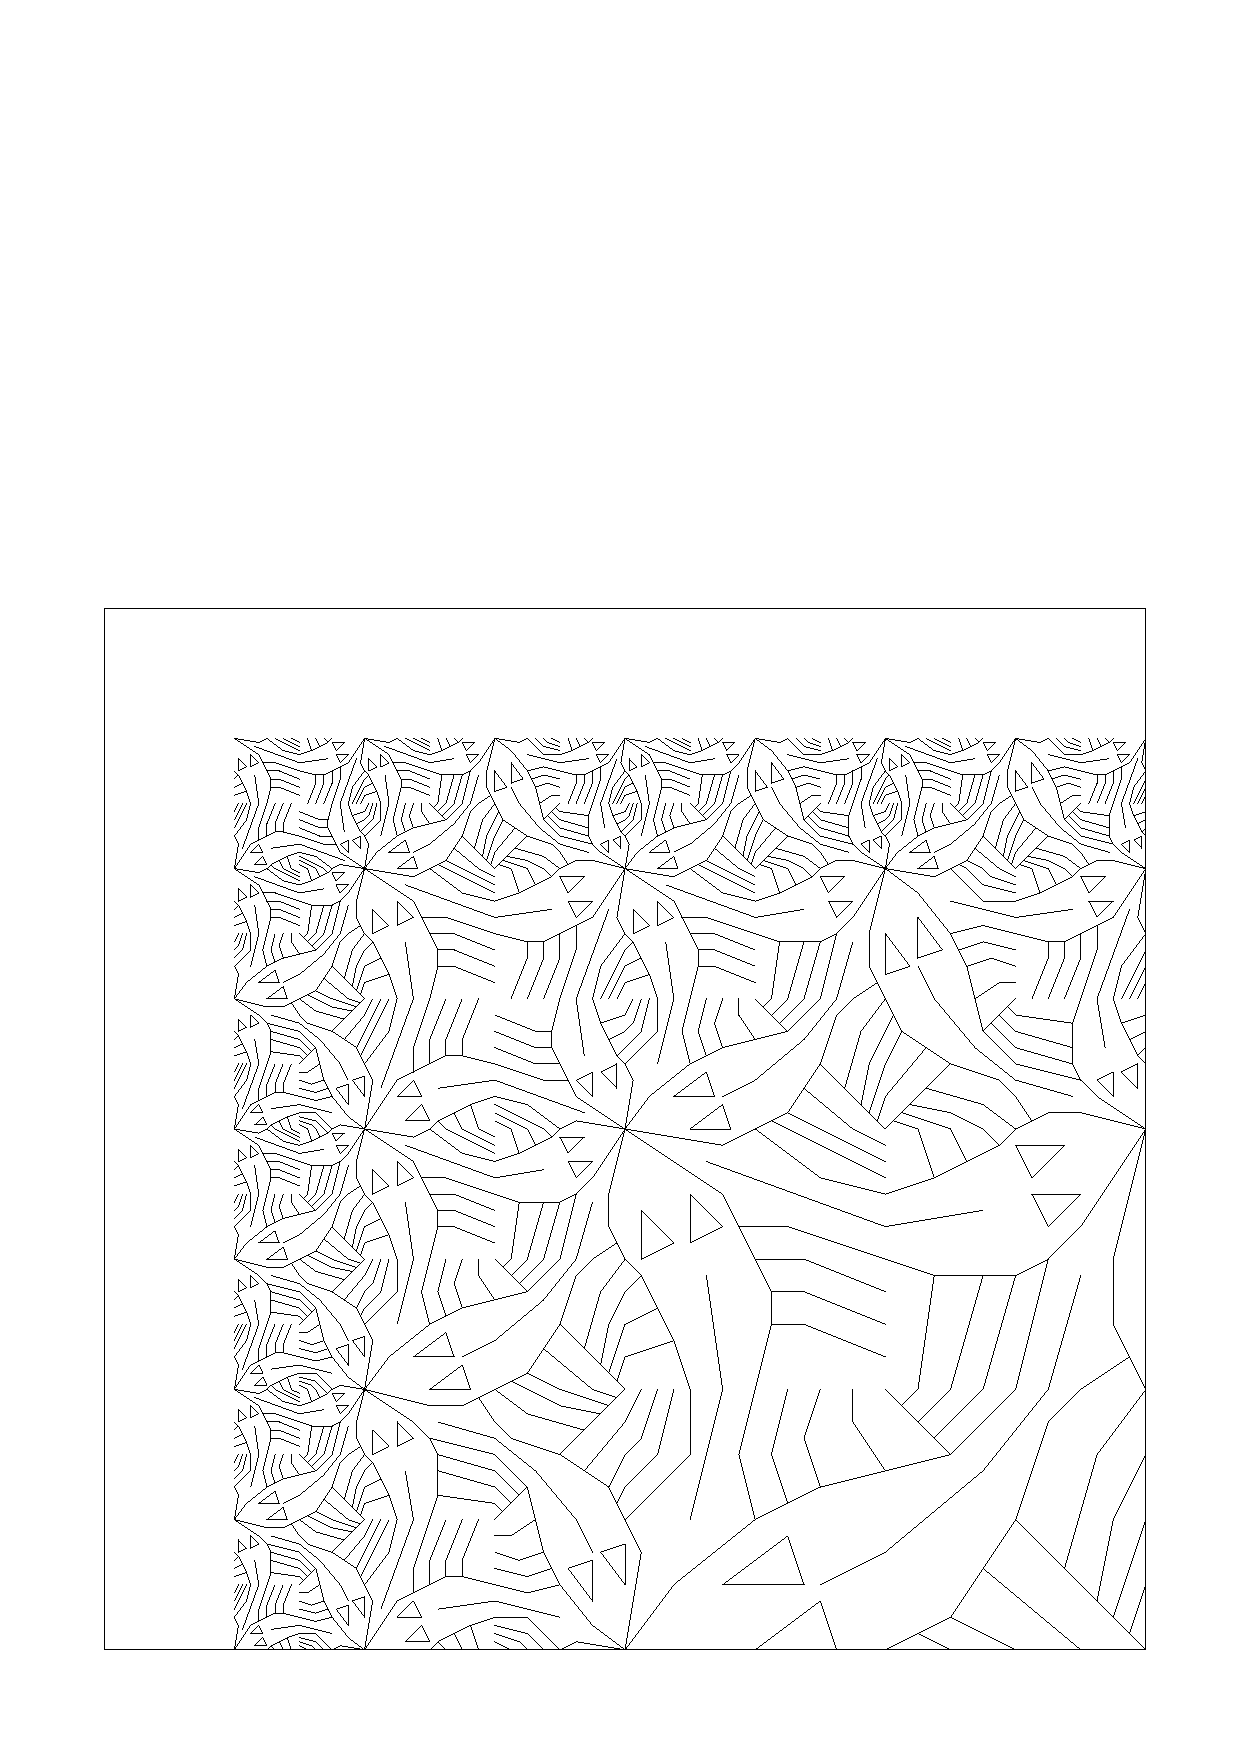
\includegraphics[width=0.5\textwidth]{./figs/fishes/pseudocorner}
            \caption{\tiny \texttt{pseudocorner = quartet(corner2, side2, rot(side2), rot(t))}}
            \label{fig:pseudocorner}
        \end{figure}

    \end{frame}

    \begin{frame}{pseudolimit}

        \begin{figure}
            \centering
            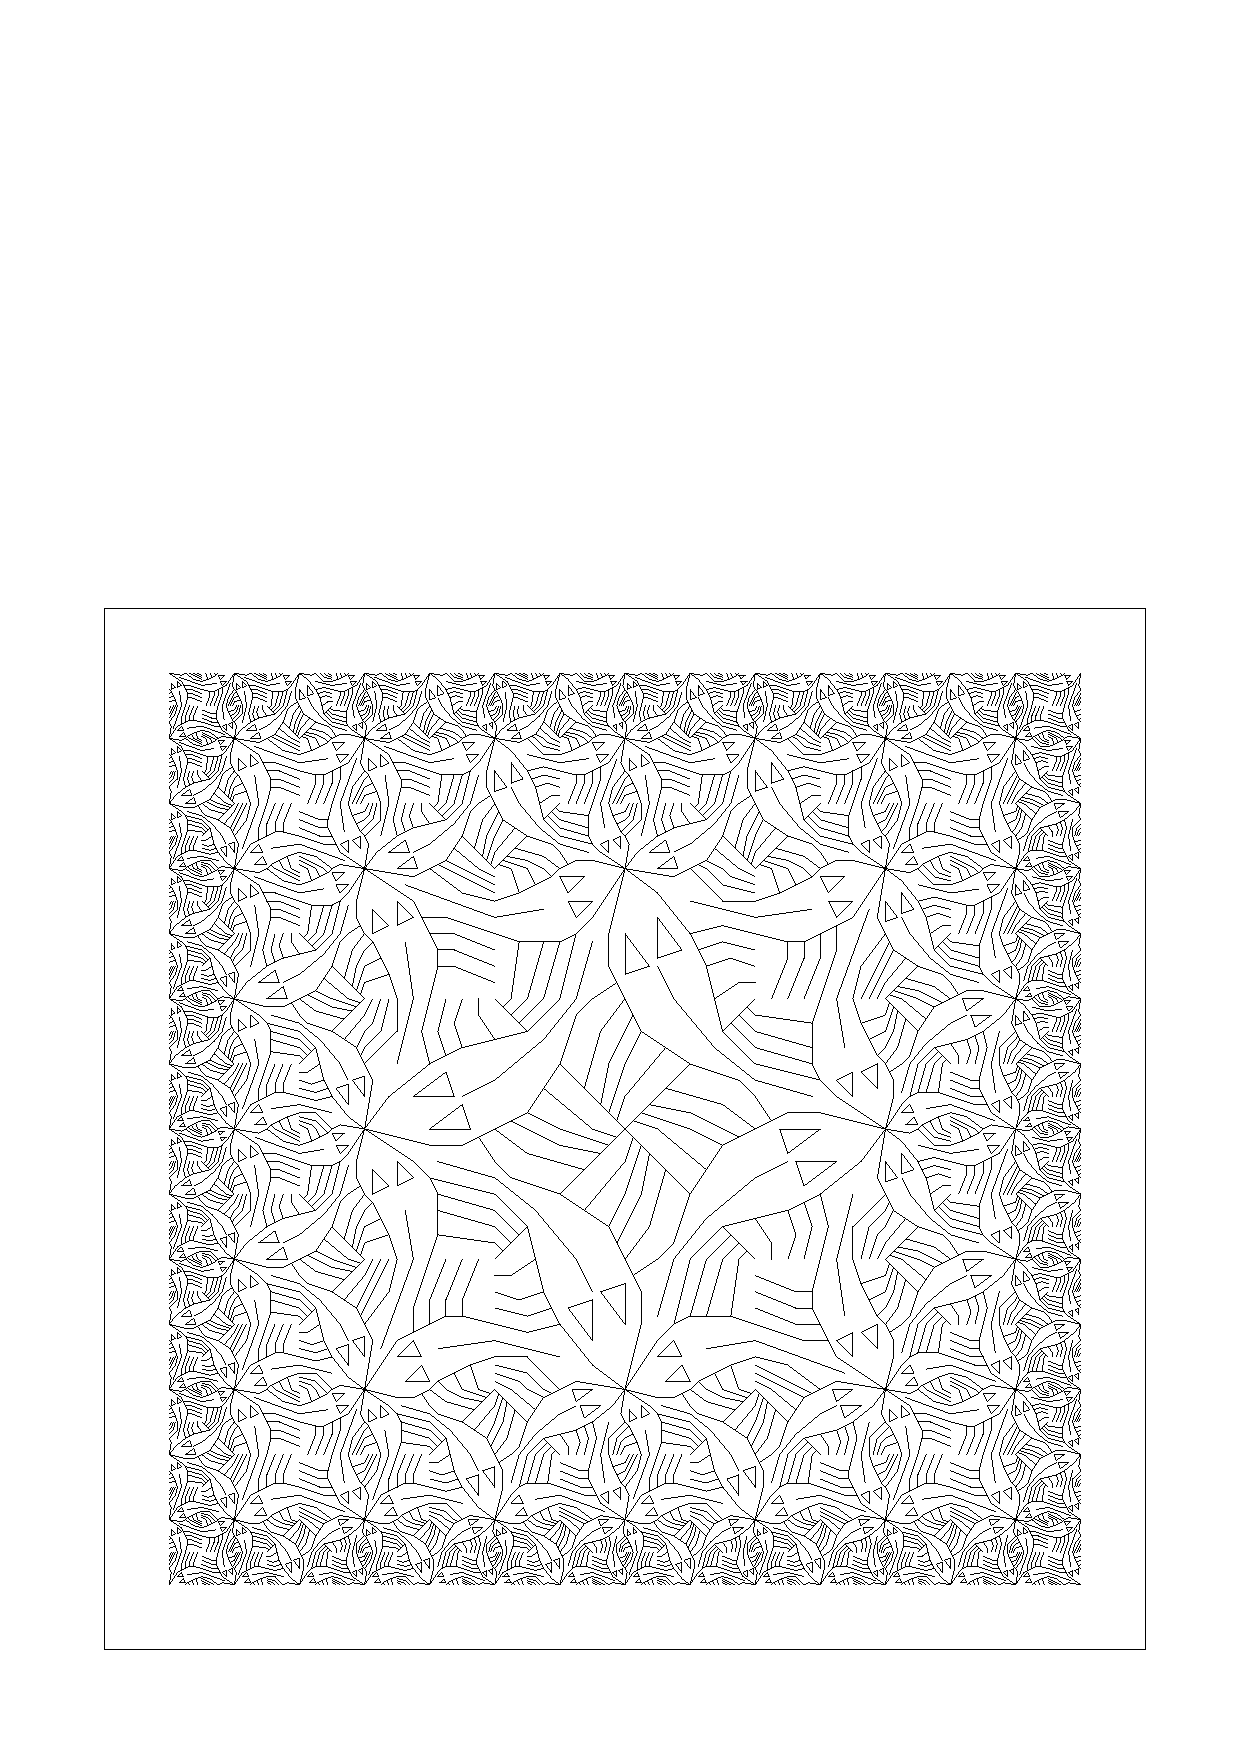
\includegraphics[width=0.5\textwidth]{./figs/fishes/pseudolimit}
            \caption{\texttt{pseudolimit = cycle(pseudocorner)}}
            \label{fig:pseudolimit}
        \end{figure}

    \end{frame}

    \begin{frame}{corner}

        \begin{figure}
            \centering
            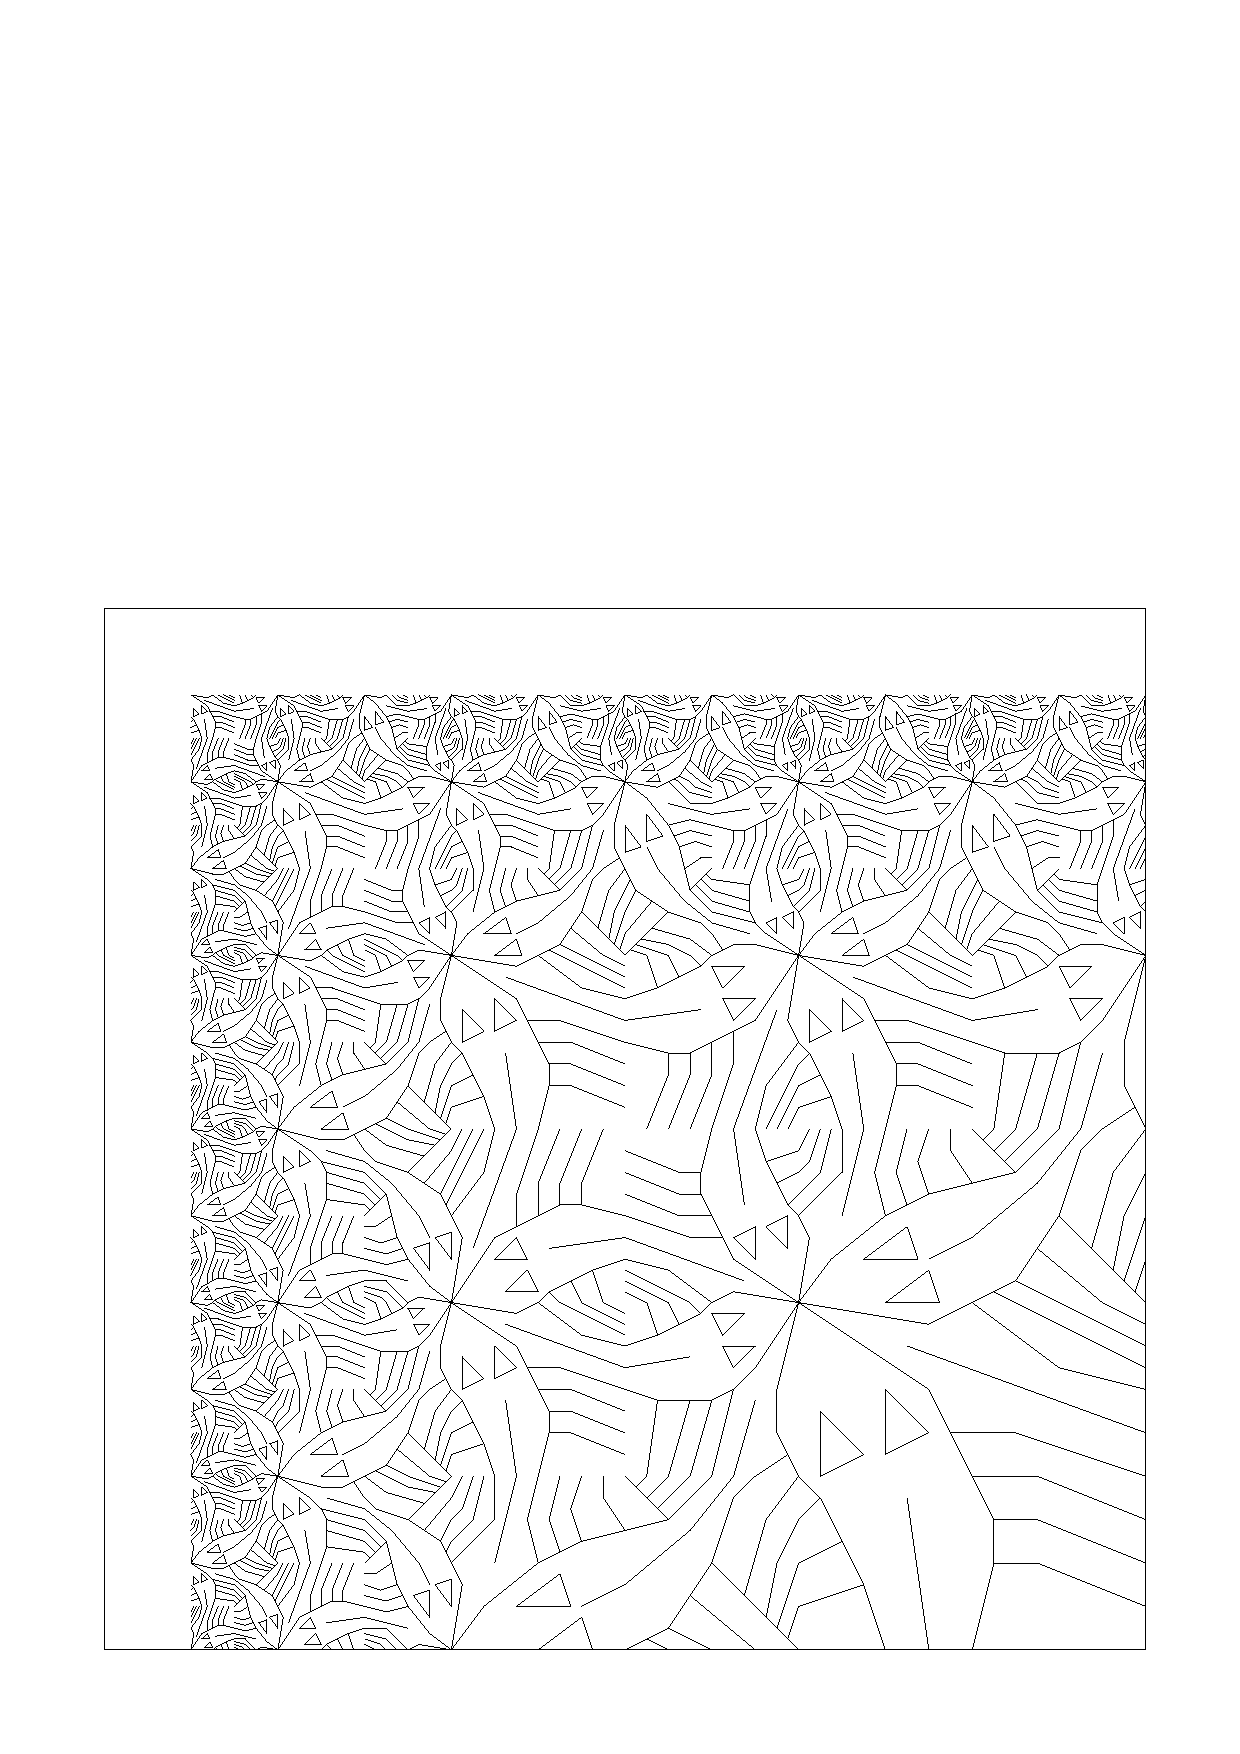
\includegraphics[width=0.5\textwidth]{./figs/fishes/corner}
            \caption{corner}
            \label{fig:corner}
        \end{figure}

    \end{frame}

    \begin{frame}{squarelimit}

        \begin{figure}
            \centering
            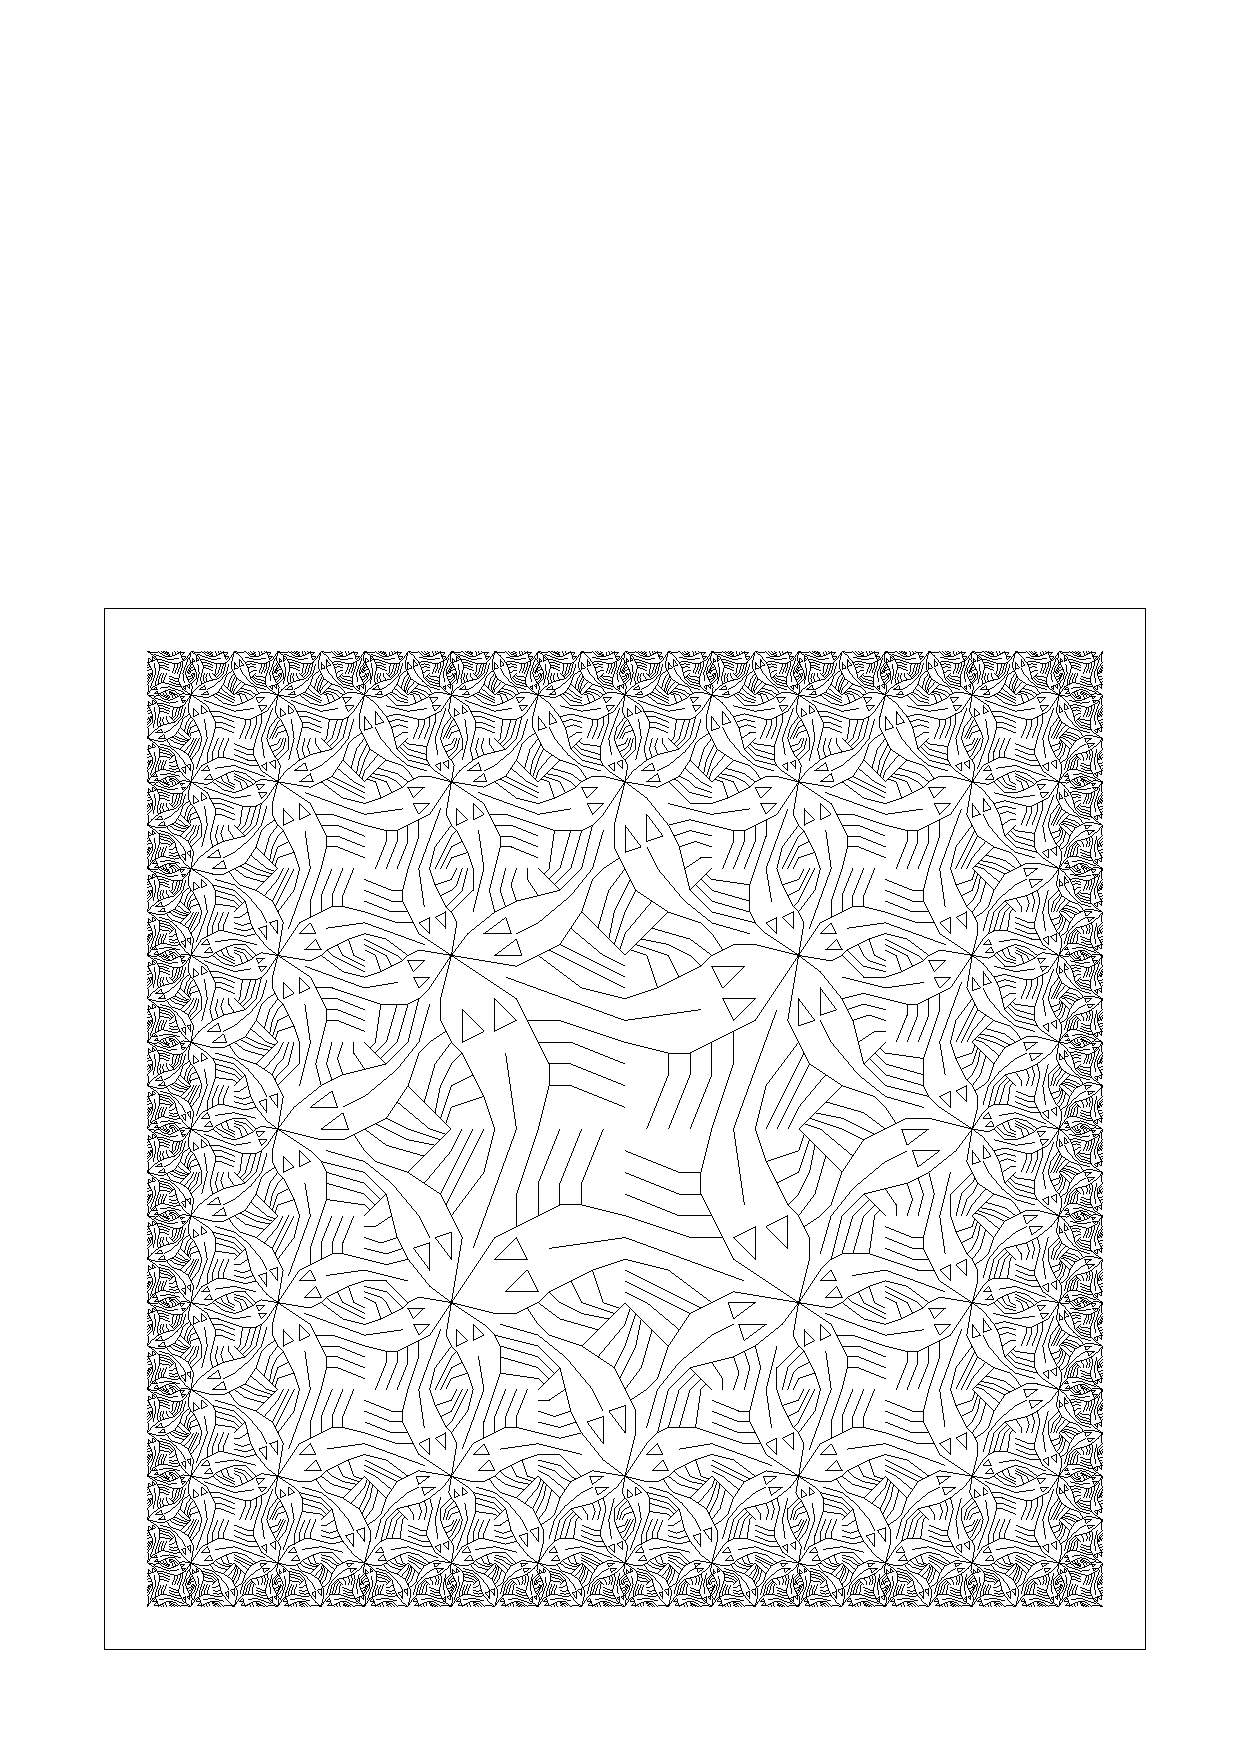
\includegraphics[width=0.5\textwidth]{./figs/fishes/squarelimit}
            \caption{squarelimit}
            \label{fig:squarelimit}
        \end{figure}

    \end{frame}

    \section{Implementation}

    \begin{frame}{Vectors}
        \begin{figure}
            \centering
            %% TODO: Include tikz picture instead
            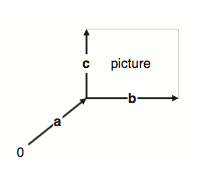
\includegraphics[width=0.5\textwidth]{./figs/vectors}
            \caption{Basic vectors}
            \label{fig:vectors}
        \end{figure}
    \end{frame}

    \begin{frame}{Implementation}
        \begin{equation*}
        over(p, q)(a, b, c) = p(a, b, c) \cup q(a, b, c)
        \end{equation*}

        \begin{equation*}
        blank(a, b, c) = \text{\{\}}
        \end{equation*}

        \begin{equation*}
        beside(p, q)(a, b, c) = p(a, \frac{b}{2}, c) \cup q(a + \frac{b}{2}, \frac{b}{2}, c)
        \end{equation*}

        \begin{equation*}
        above(p, q)(a, b, c) = p(a, b, \frac{c}{2}) \cup q (a + \frac{c}{2}, b, \frac{c}{2})
        \end{equation*}
    \end{frame}

    \begin{frame}{Implementation}
        \begin{equation*}
        rot(p)(a, b, c) = p(a + b, c, -b)
        \end{equation*}

        \begin{equation*}
        flip(p)(a, b, c) = p(a + b, -b, c)
        \end{equation*}

        \begin{equation*}
        rot45(p)(a, b, c) = p(a + \frac{b + c}{2}, \frac{b + c}{2}, \frac{c - b}{2})
        \end{equation*}
    \end{frame}

    \begin{frame}[standout]
        Demo
    \end{frame}

    \begin{frame}{Future}
        \begin{itemize}
            \item Add support for \href{https://developer.mozilla.org/en/docs/Web/SVG/Tutorial/Paths}{SVG Path}.
            %\item Build an API, in the front-end could exist something like \href{http://byob.berkeley.edu/}{Snap}
            \item Escher's ``Circuit Limit III'' picture.
        \end{itemize}

    \end{frame}

    \begin{frame}{Circuit Limit III}
        \begin{figure}
            \centering
            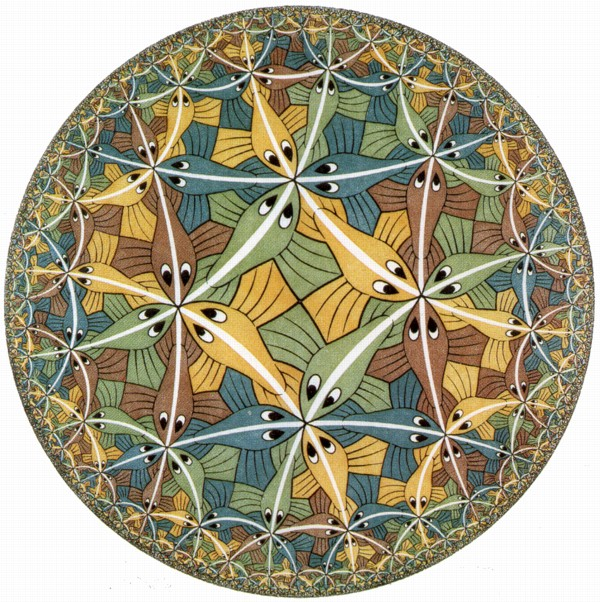
\includegraphics[width=0.5\textwidth]{./figs/Circle-Limit-III}
            \caption{Circuit Limit III}
            \label{fig:circuit_limit_iii}
        \end{figure}
        {\tiny Source: \url{http://mathstat.slu.edu/escher/upload/9/90/Circle-Limit-III.jpg}}
    \end{frame}

    \begin{frame}[standout]
        Thanks!
        \url{https://github.com/milmazz/func\_geo}
    \end{frame}

    \begin{frame}[allowframebreaks]{References}
        \bibliography{funcgeo}
        \bibliographystyle{abbrv}
    \end{frame}

\end{document}
